\section{The Underlying Physics of the Gap}\label{sec:JaoGap}
A theoretical explanation for the Jao Gap (Figure \ref{fig:JaoGap}) comes from
\citet{van2012}, who propose that in a star directly above the transition mass,
due to asymmetric production and destruction of $^{3}$He during the
proton-proton I chain (ppI), periodic luminosity variations can be induced.
This process is known as convective-kissing instability. Very shortly after the
zero-age main sequence such a star will briefly develop a radiative core;
however, as the core temperature exceeds $7\times 10^{6}$ K, enough energy will
be produced by the ppI chain that the core once again becomes convective. At
this point the star exists with both a convective core and envelope, in
addition to a thin, radiative layer separating the two. Subsequently,
asymmetries in ppI affect the evolution of the star's convective core.

While kissing instability has been the most widely adopted model to
explain the existence of the Jao Gap, slightly different mechanisms have also
been proposed. \citet{MacDonald2018} make use of a fully implicit stellar
evolution suite which treats convective mixing as a diffusive property.
\citeauthor{MacDonald2018} treat convective mixing this way in order to account
for a core deuterium concentration gradient proposed by \citet{Baraffe1997}.
Under this treatment the instability results only in a single mixing event ---
as opposed to periodic mixing events. Single mixing events may be more in line with
observations (see section \ref{sec:results} for more details on how periodic
mixing can effect a synthetic population) where there is only well documented
evidence of a single gap. However, recent work by \citet{Jao2021} which
identify an second under density of stars below the canonical gap, does leave
the door open for the periodic mixing events.

\begin{figure}
	\centering
	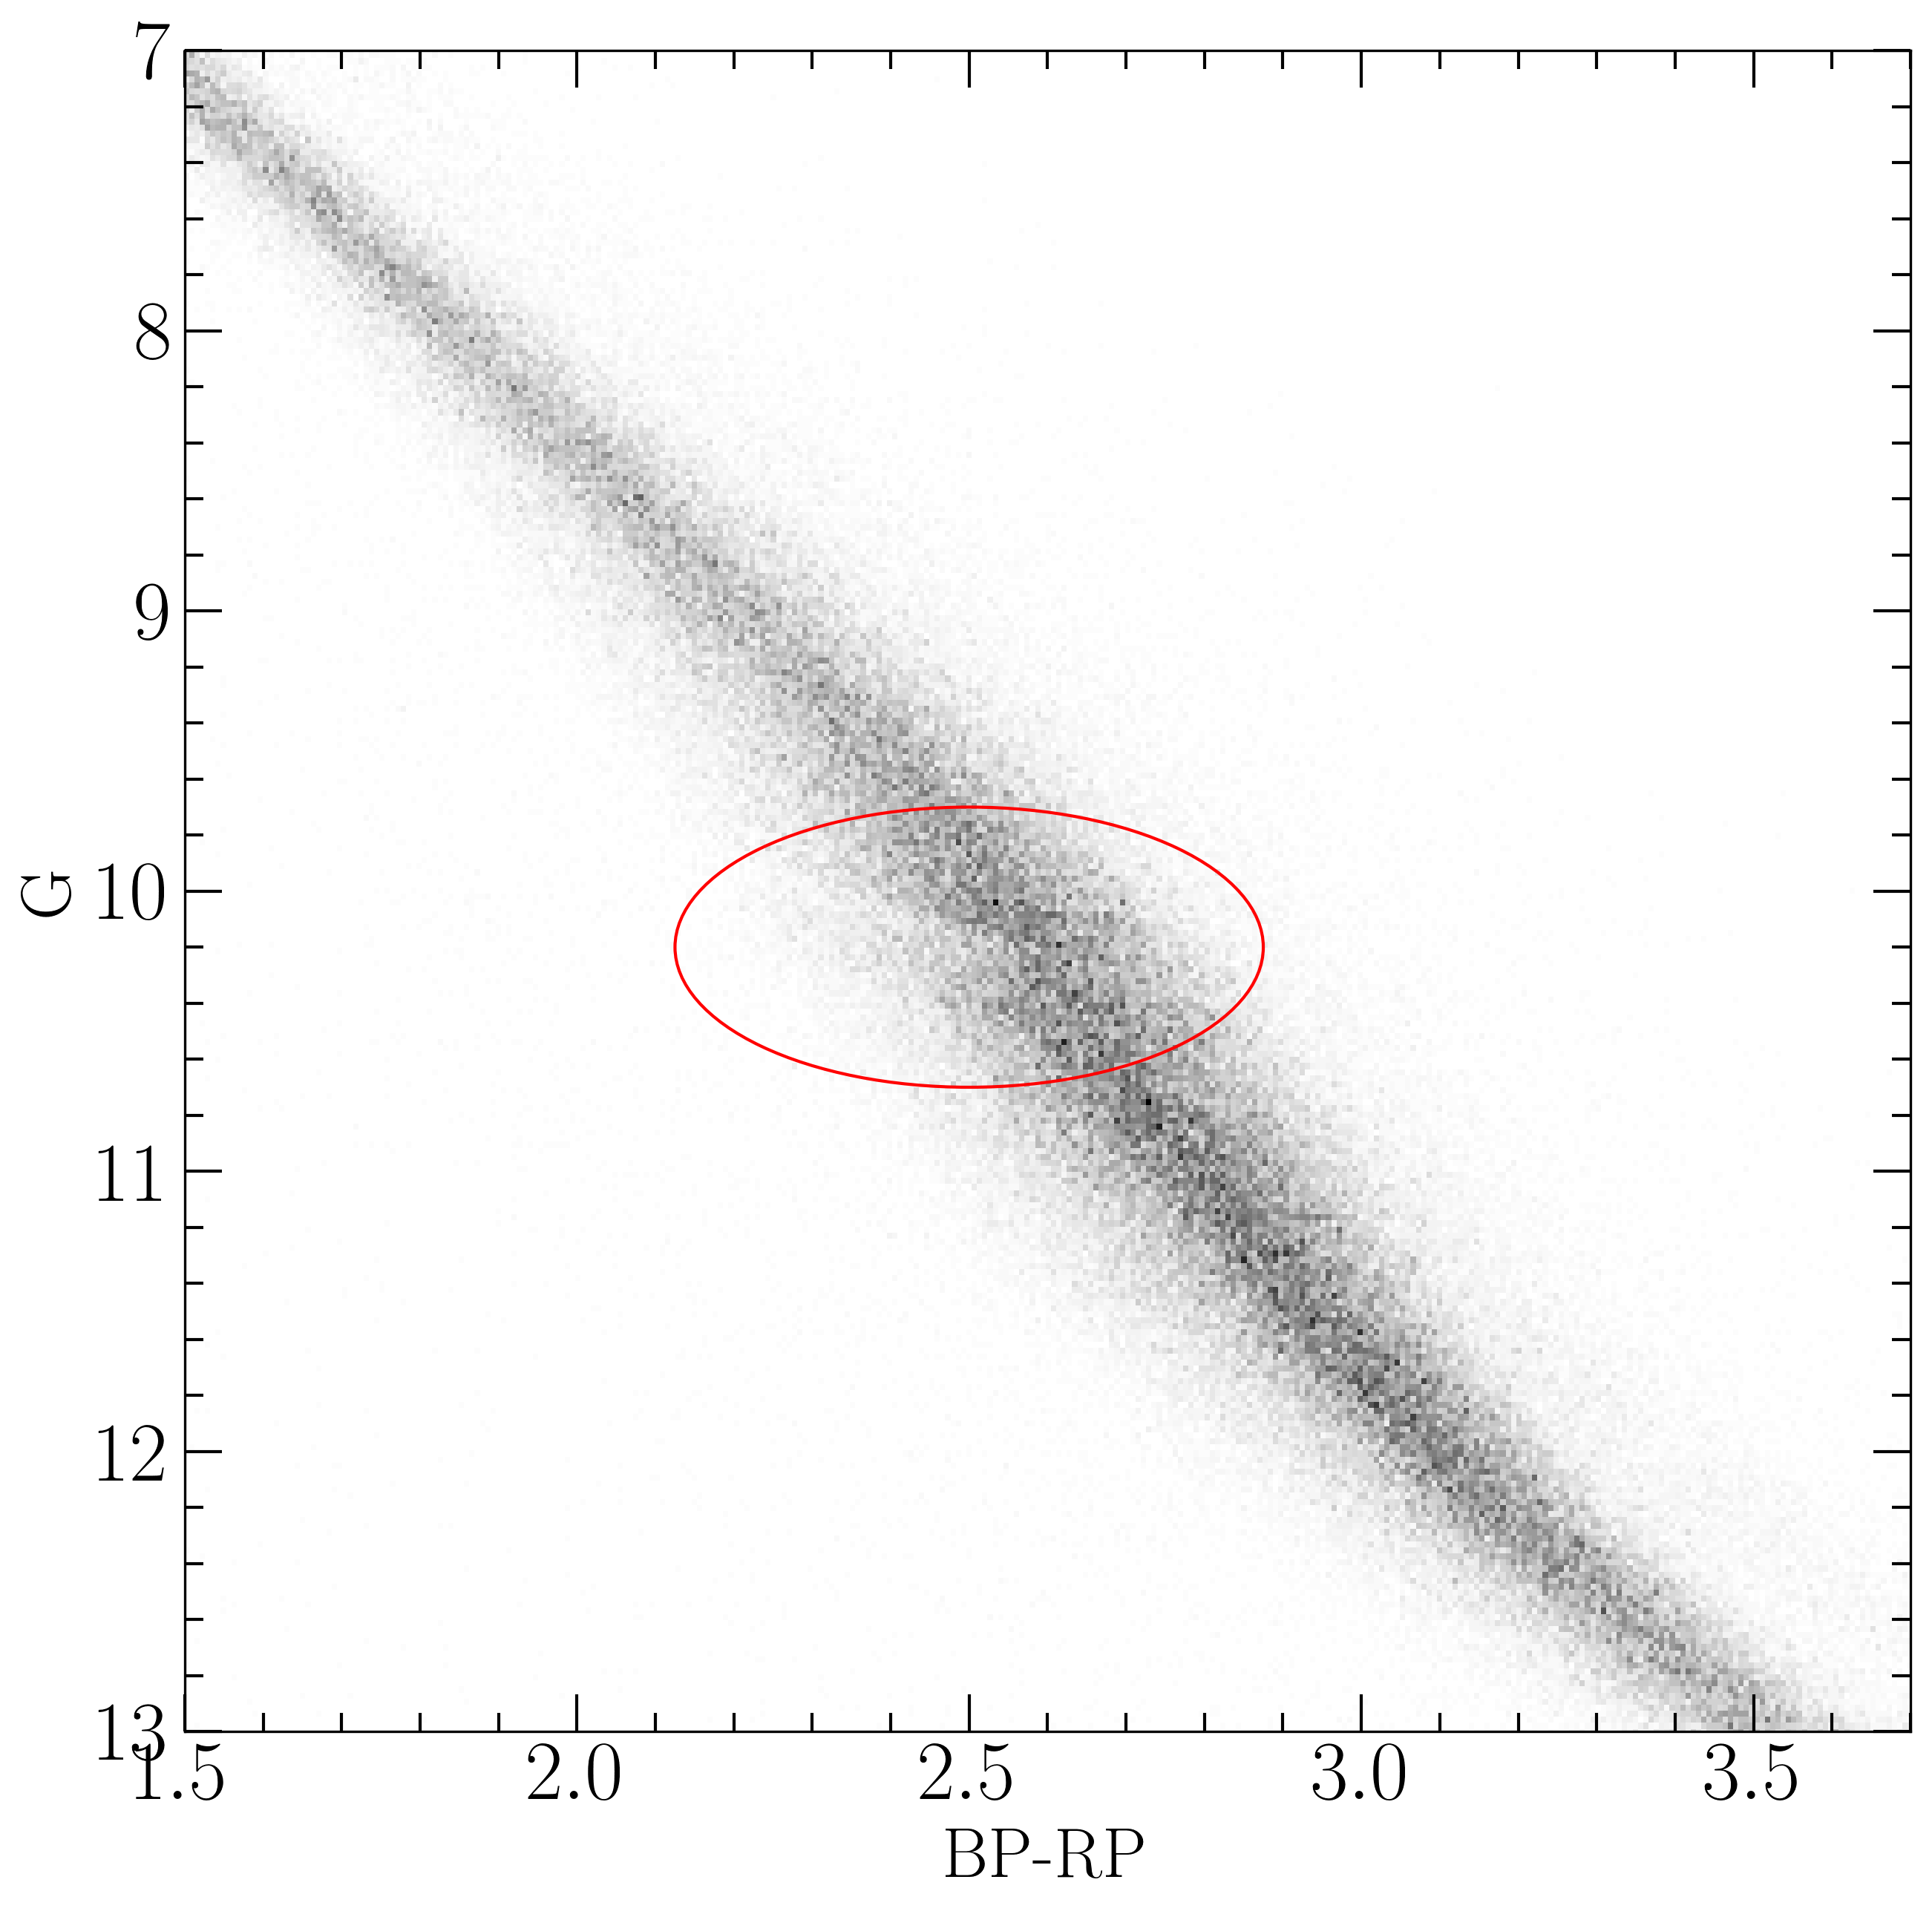
\includegraphics[width=0.85\textwidth]{figures/jaoOpacity/JaoGapEDR3.png}
	\caption{The Jao Gap (circled) seen in the Gaia Catalogue of Nearby Stars \citep{GaiaCollaboration2021}.}
	\label{fig:JaoGap}
\end{figure}

The proton-proton I chain constitutes three reactions 
\begin{enumerate} 
	\item $p + p \longrightarrow d + e^{+} + \nu_{e}$
	\item $p + d \longrightarrow \ ^{3}\text{He} + \gamma$
	\item $^{3}\text{He} + ^{3}\text{He} \longrightarrow \ ^{3}\text{He} + 2p$ 
\end{enumerate} 
Initially, reaction 3 of ppI consumes $^{3}$He at a slower rate than it is
produced by reaction 2 and as a result, the core $^{3}$He abundance and
consequently the rate of reaction 3, increases with time. The core convective
zone expands as more of the star becomes unstable to convection. This expansion
continues until the core connects with the convective envelope. At this point
convective mixing can transport material throughout the entire star and the
high concentration of $^{3}$He rapidly diffuses outward, away from the core,
decreasing energy generation as reaction 3 slows down. Ultimately, this leads
to the convective region around the core pulling back away from the convective
envelope, leaving in place the radiative transition zone, at which point
$^{3}$He concentrations grow in the core until it once again expands to meet
the envelope.  These periodic mixing events will continue until $^{3}$He
concentrations throughout the star reach an equilibrium ultimately resulting in
a fully convective star. Figure \ref{fig:Kippenhan1} traces the evolution of a
characteristic star within the Jao Gap's mass range.

\begin{figure*}
	\centering
	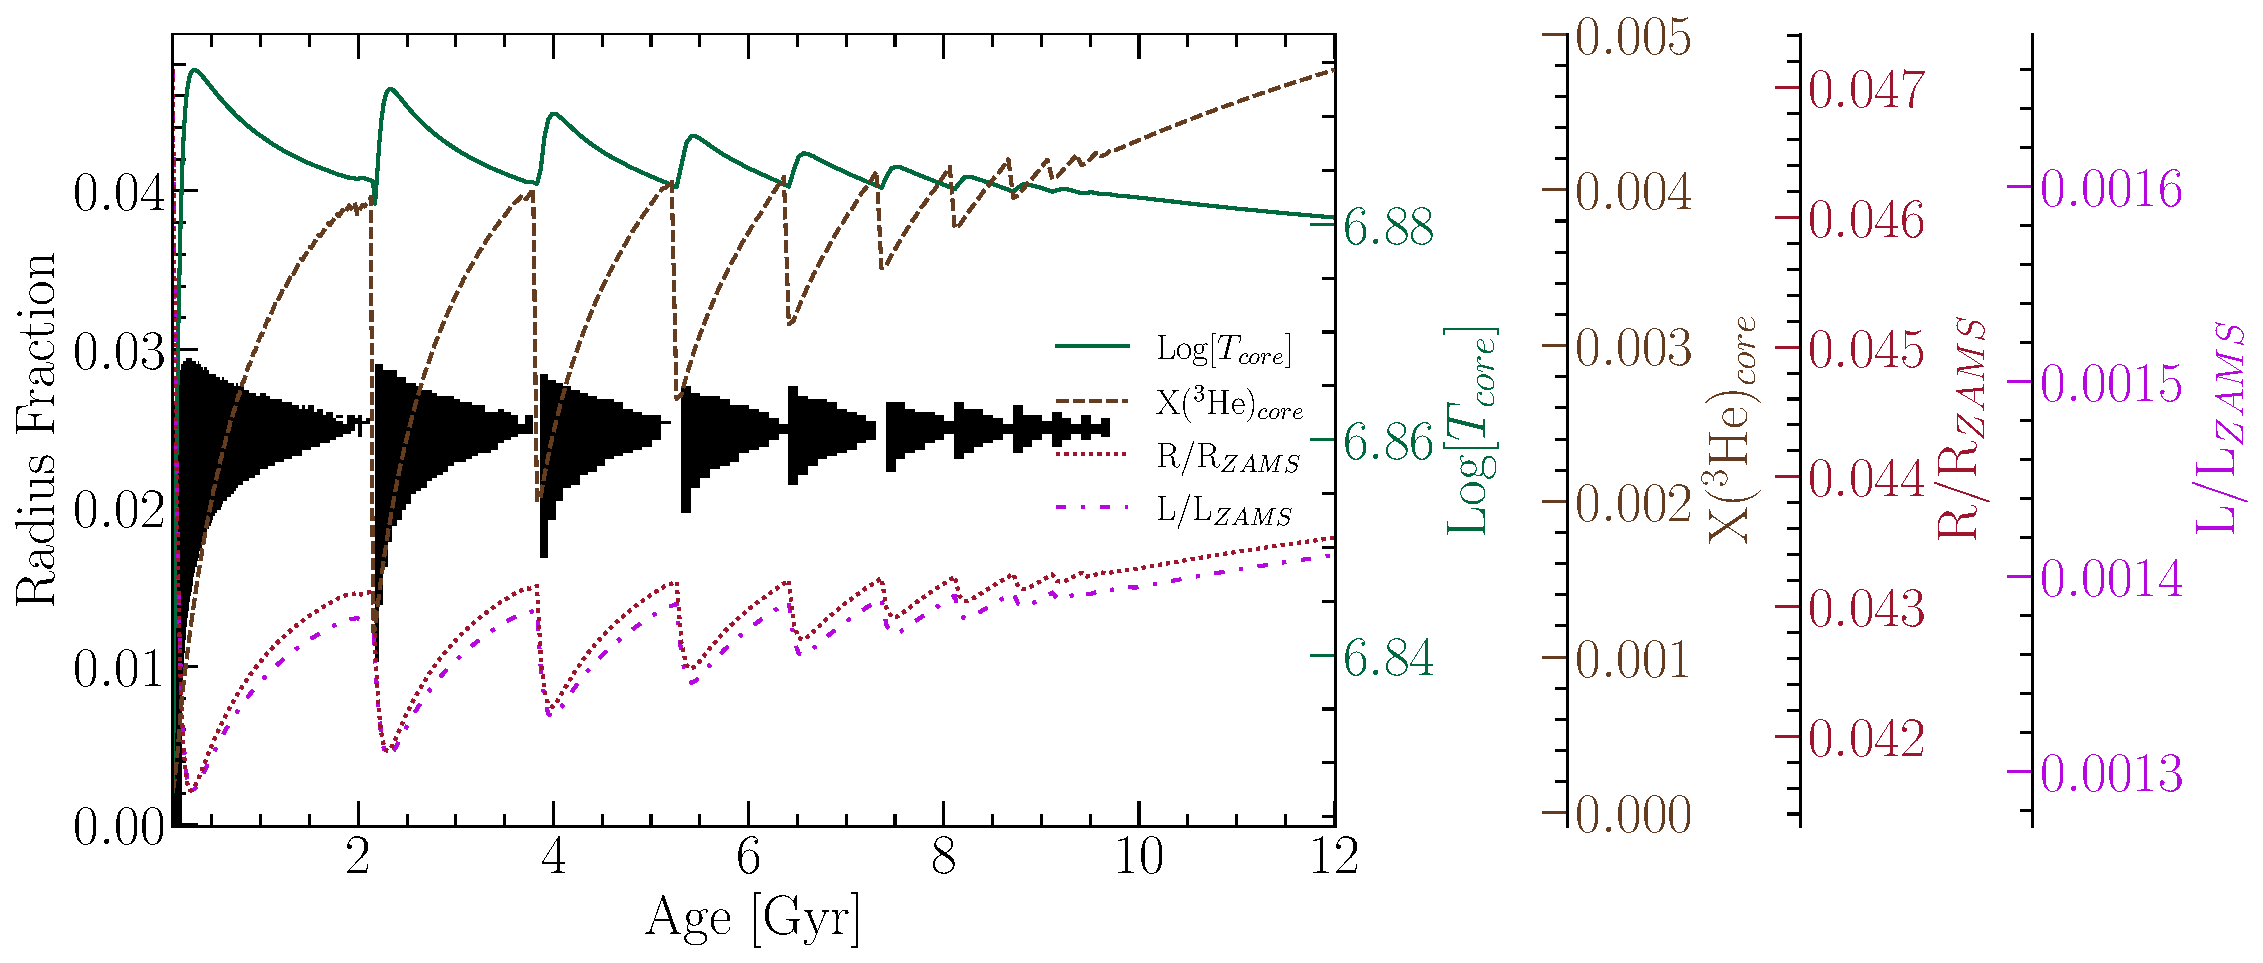
\includegraphics[width=0.95\textwidth]{figures/jaoOpacity/Kippenhan.pdf}
	\caption{Diagram for a characteristic stellar model of 0.35625 $M_{\odot}$
	which is within the Jao Gap's mass range. The black shaded regions denote
	whether, at a particular model age, a radial shell within the model is
	radiative (with white meaning convective). The lines trace the models core
	temperature, core $^{3}$He mass fraction, fractional luminosity wrt. the
	zero age main sequence and fractional radius wrt. the zero age main
	sequence.}
	\label{fig:Kippenhan1}
\end{figure*}


\subsection{Efforts to Model the Gap}
Since the identification of the Gap, stellar modeling has been
conducted to better constrain its location, effects, and exact cause.
Both \citet{Mansfield2021} and \citet{Feiden2021} identify that the Gap's mass
location is correlated with model metallicity --- the mass-luminosity
discontinuity in lower metallicity models being at a commensurately lower mass.
\citet{Feiden2021} suggests this dependence is due to the steep relation of
the radiative temperature gradient, $\nabla_{rad}$, on temperature and, in turn,
on stellar mass.

\begin{align}\label{eqn:radGrad}
	\nabla_{rad} \propto \frac{L\kappa}{T^{4}}
\end{align}

As metallicity decreases so does opacity, which, by Equation \ref{eqn:radGrad},
dramatically lowers the temperature at which radiation will dominate energy
transport \citep{Chabrier1997}. Since main sequence stars are virialized the
core temperature is proportional to the core density and total mass. Therefore,
if the core temperature where convective-kissing instability is expected
decreases with metallicity, so too will the mass of stars which experience such
instabilities.

% \begin{align}\label{eqn:TMRelation}
% 	T_{c} \propto \rho_{c}M^{2}
% \end{align}

The strong opacity dependence of the Jao Gap begs the question: what is
the effect of different opacity calculations on Gap properties.
As we can see above, changing opacity should affect the Gap's location in the
mass-luminosity relation and therefore in a color-magnitude diagram. Moreover,
current models of the Gap have yet to locate it precisely in the CMD
\citep{Feiden2021} with an approximate 0.16 G-magnitude difference between the
observed and modeled Gaps. Opacity provides one, as yet unexplored, parameter
which has the potential to resolve these discrepancies.
